% Investigate, Recommend or Escalate: A Rule-Constrained Reinforcement Learning Agent
% for IT Incident Triage under Ambiguous Evidence
%
% Laid out on the department template (_U_Proposal_Report_template_2026_CS_DS_Undergraduate.zip),
% the same layout as the proposal in ../proposal/.
%
% Build from this folder:   ..\..\tools\tectonic.exe Opol_Charis_Thesis.tex
%
% Layout:
%   Opol_Charis_Thesis.tex    preamble, title page, chapter order, bibliography
%   chapters/                 one file per chapter (body text only)
%   images/                   figures
%   citations/references.bib  all references, shared by every chapter

\documentclass[12pt]{report}
\usepackage{appendix}
\usepackage[utf8]{inputenc}
\usepackage{graphicx}
\usepackage{color}
\usepackage[table]{xcolor}
\usepackage{longtable}
\usepackage[paper=a4paper,bottom=2cm,footskip=0.25cm,top=2cm,headsep=0.25cm,rmargin=2cm,lmargin=2cm]{geometry}
\usepackage{tabularx}
\usepackage{booktabs}
\usepackage{float}
\usepackage[parfill]{parskip}
\usepackage{enumitem}
\usepackage{amsmath}
\usepackage{amssymb}
\usepackage{cite}
\usepackage[hyphens]{url}

\usepackage{hyperref}
\usepackage{mathtools}
\hypersetup{
    colorlinks=false,
    linktoc=all,
    linkcolor=blue,
}

\setcounter{secnumdepth}{3}    % Number subsubsections in the chapters
\setcounter{tocdepth}{3}       % Put subsubsections in the table of contents

\graphicspath{{images/}}
\emergencystretch=1.5em
\setlist{itemsep=0.4em}

% ---------------------------------------------------------------------------
% Table helpers (Chapters Two and Three)
% ---------------------------------------------------------------------------
\newcommand{\cellyes}{$\checkmark$}
\newcommand{\cellpart}{$\circ$}
\newcommand{\cellno}{--}
\newcolumntype{L}{>{\raggedright\arraybackslash}X}

%%%% Student data fields %%%%
\newcommand\theResearchTopic{\textit{Investigate, Recommend or Escalate: A Rule-Constrained Reinforcement Learning Agent for IT Incident Triage under Ambiguous Evidence}}

\newcommand\theStudentName{\textit{OPOL CHARIS}}
\newcommand\theStudentRegNo{\textit{S24B23/003}}
\newcommand\theStudentNo{\textit{B29654}}
\newcommand\theStudentEmail{\textit{charisopol@gmail.com}}
\newcommand\theStudentPhoneNo{\textit{0765821211}}

\newcommand\theSpecializationTrack{\textit{Artificial Intelligence and Robotics}}

\newcommand\thePrimaryAdvisor{\textit{\textcolor{red}{IAN RAYMOND OSOLO}}}

\newcommand\theProgrameAward{Bachelor of Science in Computer Science}
\newcommand\theTheDocumentType{report}
\newcommand\theFinalOutputDocument{Degree}

\newcommand\theFaculty{Faculty of Engineering Design \& Technology}
\newcommand\theDepartment{Department of Computing \& Technology}

\newcommand\theVersionDate{\textit{\textcolor{red}{[Enter Version Date]}}}

\newcommand\makLogo{
\includegraphics[scale=.3]{../proposal/images/logos/UCU-Logo.png}}


\pagenumbering{roman}
\begin{document}
    %%---- Title page
    \begin{titlepage}
        \centering
        \makLogo  \\
         \theDepartment \\
    	\vspace{1cm}
        \Large{
            \theResearchTopic \\

            \vspace{.5cm}
            \textit{By}\\
            \vspace{.5cm}
            \theStudentName\\

            Reg No: \theStudentRegNo, Student No: \theStudentNo  \\
            E-mail: \theStudentEmail, Phone No:  \theStudentPhoneNo\\

            \vspace{1cm}

            A \theTheDocumentType~submitted to the \theFaculty~for the study leading to the \theFinalOutputDocument~in partial fulfilment of the requirements for the award of \textbf{\theProgrameAward}~of Uganda Christian University \\

            \vspace{1cm}

            SPECIALIZATION TRACK: \theSpecializationTrack\\
              \vspace{1cm}
            \thePrimaryAdvisor \\

             \vspace{1cm}
            \theVersionDate \\
       }
    \end{titlepage}

\tableofcontents
\listoffigures
\listoftables

% ---------------------------------------------------------------------------
% Chapters: comment a line out to leave a chapter out of the build.
% ---------------------------------------------------------------------------
\chapter{Introduction}
\label{ch:chapter-01}
\pagenumbering{arabic}
% Chapter One: Introduction
% Compiled through main.tex; do not compile this file on its own.

\chapterheading{ONE}{INTRODUCTION}

This chapter introduces a study of how an automated agent should decide what to do when the evidence about an IT incident is incomplete or conflicting. It presents the background to IT incident triage, states the research problem, and sets out the objectives, research questions and hypotheses of the study. It then defines the scope, significance and justification of the research, describes the conceptual framework, and defines the key terms used in the chapters that follow.

\section{Background to the Study}

Organisations depend on IT services that are expected to remain available, and incident management is the process that restores those services when they fail. An incident is an unplanned interruption or outage of a service~\cite{chen2020}. Chen et al.\ describe incident management as the process of detecting a service problem, creating an incident, determining its cause, restoring the service, and capturing knowledge to prevent a recurrence~\cite{chen2020}. Failures that are handled slowly reduce system availability and can lead to financial loss and user dissatisfaction~\cite{chen2020,remil2024}. The speed and quality of the decisions made early in this process therefore affect how long a service stays degraded.

Incident triage is the stage at which a reported incident is assessed and directed towards resolution. Chen et al.\ define triage as engaging the team responsible for investigating the problem~\cite{chen2020}. Remil et al.\ use the term more broadly to cover the prioritisation, assignment and classification of incidents, together with the identification of duplicates~\cite{remil2024}. Both descriptions present triage as a set of decisions made before the root cause is known. This study adopts the same view and treats ambiguity-aware IT incident triage as the task of deciding what should happen next to an incident whose cause is still uncertain.

Researchers and practitioners have moved triage from manual and rule-based processing towards learned models. Traditional IT management relied on expert systems and rule-based engines, which Remil et al.\ report as limited in adaptiveness, efficiency and scalability~\cite{remil2024}. Artificial Intelligence for IT Operations (AIOps) addresses these limits with machine learning models that classify, prioritise and assign incidents from reports, logs and metrics~\cite{chen2020,remil2024}. Large language models have extended this work to root cause analysis and the generation of mitigation suggestions from incident reports~\cite{zhang2025}. These approaches differ in what they hand to the person responsible. AI-assisted diagnosis proposes a cause, decision support recommends an action for a person to approve, automated execution carries the action out, and escalation passes the decision to a person. The literature is uneven across the four: Zhang et al.\ observe that automation efforts mainly stop at incident triage or solution recommendation, and that work on automatic execution is limited and its practical effectiveness remains to be verified~\cite{zhang2025}. The move from recommending to acting is therefore the least settled part of AI-assisted incident handling.

Triage decisions are difficult because the evidence available at the time of the decision is often incomplete or conflicting. In their two-year study of incident management at Microsoft, Chen et al.\ found that symptoms are sometimes insufficient to identify the responsible team, since distinct problems can produce similar symptoms, and that incidents are consequently reassigned several times~\cite{chen2020}. The same study attributes delays to incomplete knowledge of service dependencies and imprecise assessment of resource health~\cite{chen2020}. Remil et al.\ likewise note that data in real IT environments is commonly noisy and incomplete, and they list robustness to such data as a requirement for AIOps solutions~\cite{remil2024}. Many triage models nevertheless treat the task as a single prediction over the incident report, evaluated with classification or ranking metrics~\cite{remil2024}. A model of this kind returns an answer for every report and has no means to state that more evidence is needed before it can answer. Ambiguity is therefore a property of the triage task that a single-step prediction does not represent.

Reinforcement learning offers a way to treat triage as a sequence of decisions and not as one prediction. In reinforcement learning, an agent learns a policy by acting in an environment and receiving rewards that reflect the consequences of its actions~\cite{sutton2018}. When the agent cannot observe the true state of the environment, it can choose actions whose purpose is to obtain information, and it must weigh the cost of that information against its value~\cite{kaelbling1998}. Janisch et al.\ applied this idea to classification with costly features, where an agent learns which features to acquire before it commits to a decision~\cite{janisch2019}. Reinforcement learning and related sequential methods have also been applied to incident handling. In IT operations, Wang et al.\ used reinforcement learning to reduce the number of questions put to engineers during root cause analysis~\cite{wang2023hrlhf}. In cybersecurity, Ren et al.\ trained an agent to select response strategies for security incidents~\cite{ren2025}, Dunsin et al.\ modelled post-incident malware investigation as a Markov decision process~\cite{dunsin2025}, Kim and D\'{a}n developed policies for choosing which alerts to investigate~\cite{kim2025}, and Hammar and Li planned responses when the model of the incident is itself uncertain~\cite{hammar2025}. These studies show that incident handling can be framed as a sequential decision problem and that the gathering of evidence can be made part of it. Their agents choose among responses or investigative steps, however, and the studies leave open how such an agent should behave when it is not permitted, or not well placed, to act.

An agent that recommends actions on production systems must respect operational constraints, and a reward signal alone does not ensure this. Reinforcement learning algorithms find policies that maximise reward but do not guarantee safe behaviour during learning or execution~\cite{alshiekh2018}, and penalising undesirable actions in the reward does not guarantee that the agent never selects them~\cite{konighofer2025}. Safe reinforcement learning addresses this by requiring policies to respect safety constraints as well as maximise return~\cite{garcia2015}. One group of methods constrains the expected cumulative cost of a policy~\cite{achiam2017,wachi2024}. Many practical constraints, however, are instantaneous and must hold at every step~\cite{zhao2023}. Shielding is designed for this case: a separate component monitors each action the agent proposes and overrides it only when the action would violate a given specification~\cite{alshiekh2018}. The guarantee a shield provides is limited to the specification and the environment model from which it is built~\cite{konighofer2025}. For incident handling, Remil et al.\ state the corresponding requirement directly: automatic healing actions need to be executed safely~\cite{remil2024}. Two recent studies act on this requirement in security settings. Alauthman et al.\ propose a reinforcement learning agent with an explicit safety shield for incident response in industrial control systems~\cite{alauthman2026}, and Hammar et al.\ check the actions proposed by a language model against system constraints before they are used~\cite{hammar2026llm}. A rule of this kind in IT support might, for example, forbid restarting a production database without approval.

Human experts remain necessary when ambiguity cannot be resolved or when a decision falls outside what the agent is permitted to do. Selective prediction gives a model the option to abstain when it is not sufficiently confident~\cite{geifman2019}, and learning to defer extends this by training the model to decide when a human decision-maker should take over~\cite{madras2018}. This research shows that deferral carries its own difficulties. Learning when to defer normally requires data about the expert's decisions~\cite{hemmer2023}, and the way a deferral is communicated affects the accuracy of the person who receives it~\cite{bondi2022}. Joshi et al.\ extended deferral to sequential settings, in which the choice to defer affects later states~\cite{joshi2023}. Guidance on AI risk management also recognises that an AI system may decide autonomously, defer to a human expert, or act as an additional opinion, and it requires that these roles be clearly defined~\cite{nist2023}. Recent work outside IT operations supports making escalation an explicit and governed decision. Pacella et al.\ found that a language-model agent without a guardrail failed to escalate cases that policy required a human to approve~\cite{pacella2026}, and Bachar et al.\ treated escalation in content moderation as a cost-aware decision based on uncertainty~\cite{bachar2026}. A recent preprint adds that human attention is finite, so an agent that escalates too often may weaken the oversight it relies on~\cite{turan2026}. Escalation is consequently a decision with costs in both directions, and not a safe default.

These bodies of work have developed largely apart, and where they meet they do so in pairs. AIOps research has concentrated on predicting the category, owner or cause of an incident. Studies of information gathering let an agent choose between looking further and deciding~\cite{janisch2019,kim2025}, while studies of deferral let it choose between deciding and handing over~\cite{madras2018,joshi2023}. Shielding has been demonstrated mainly in control and robotics tasks~\cite{alshiekh2018,achiam2017,zhao2023}, and the shielded agent proposed for incident response selects responses and does not choose whether to investigate or escalate~\cite{alauthman2026}. The studies reviewed for this research do not examine an agent for IT incident triage that chooses among gathering further diagnostic information, recommending a permitted action, and escalating to a human expert, with its proposals checked by an independent set of operational rules. Nor do they evaluate such an agent as the ambiguity of its evidence is varied. This study addresses that opportunity. It proposes to design a rule-constrained reinforcement learning agent for ambiguity-aware IT incident triage and to evaluate it in a controlled simulation. Part of the study will be carried out with the Directorate of University ICT Services at Uganda Christian University, whose incident-handling practice is expected to inform the scenarios and operational constraints that the simulation represents.

\section{Problem Statement}

IT support teams must decide how to handle an incident before they know its cause. The evidence available at that point is often incomplete, and different observations can point towards different explanations~\cite{chen2020,remil2024}. A member of IT staff facing such an incident can investigate further, apply a likely remedy, or pass the incident to someone better placed to resolve it. Each choice has a cost. Further investigation takes time, a wrong remedy can prolong or worsen the incident, and unnecessary escalation consumes the attention of senior staff.

Existing automated approaches address parts of this decision but not the choice among its options. Triage models commonly produce one prediction per incident report~\cite{chen2020,remil2024}, which does not allow the model to ask for more evidence. Sequential methods have been applied to incident response and investigation, mostly in cybersecurity~\cite{ren2025,dunsin2025,kim2025,hammar2025}, and some of them decide what evidence to gather. A few studies of security alert triage also let the agent escalate or defer an alert to an analyst~\cite{sahin2026,kovtun2026}, but their agents close or escalate alerts and do not recommend a remedy, and a systematic review of 34 studies found escalation to a person in only seven of them~\cite{opol2026slr}. Learning to defer provides a principled basis for handing decisions to humans~\cite{madras2018,joshi2023}, but it treats the choice as one between deciding and deferring, without the option of gathering information first. Shielding and constrained reinforcement learning provide ways to restrict an agent's actions~\cite{alshiekh2018,achiam2017}, and a shielded agent has been proposed for incident response in industrial control systems~\cite{alauthman2026}. Only three of the 34 studies in the systematic review report what happens when such a mechanism blocks a decision~\cite{opol2026slr}, and the reviewed literature does not report how the mechanism behaves when the agent can also investigate or escalate.

The gap this study investigates is therefore specific, and Chapter Two sets it out in five parts. The reviewed literature offers no controlled environment for IT service incidents in which ambiguity can be varied. It does not show whether one policy can learn to choose among investigating, recommending and escalating, or how an independent rule-based mechanism interacts with that choice. It has not measured decision quality, investigation cost, escalation behaviour and constraint compliance together for one agent, nor has it shown how an agent's mix of decisions changes as evidence becomes scarcer or more contradictory. The study does not claim that constraining a learned incident-handling agent is new, or that no related work exists beyond the literature reviewed. This study proposes to build a simulated triage environment, informed in part by work with the Directorate of University ICT Services at Uganda Christian University, in which the question can be tested, and to compare a rule-constrained reinforcement learning agent with baseline decision policies. Whether the agent improves on those baselines is a question for the experiments and not an assumption of the study.

\section{Research Objectives}

\subsection{General Objective}

To design and evaluate a rule-constrained reinforcement learning agent for ambiguity-aware IT incident triage that learns when to gather additional diagnostic information, recommend permitted actions, or escalate incidents to a human expert.

\subsection{Specific Objectives}

\begin{enumerate}
  \item To identify and model IT incident triage scenarios involving incomplete, uncertain, or conflicting diagnostic evidence.
  \item To design a reinforcement learning environment in which an agent can request diagnostic information, recommend permitted actions, or escalate incidents.
  \item To implement an independent rule-based safety mechanism that checks proposed actions against predefined operational constraints.
  \item To evaluate the proposed approach against selected baseline decision policies using measures of decision quality, investigation efficiency, escalation behaviour, and constraint compliance.
  \item To assess the robustness of the agent under different levels of ambiguity and missing diagnostic information.
\end{enumerate}

\section{Research Questions}

This study will answer the following research questions:

\begin{enumerate}
  \item How can ambiguous IT incident triage scenarios involving incomplete or conflicting diagnostic evidence be represented in a controlled environment?
  \item How can reinforcement learning support decisions about gathering diagnostic information, recommending permitted actions, and escalating incidents to a human expert?
  \item How effectively can a rule-based safety mechanism prevent actions that violate predefined operational constraints?
  \item How does the proposed approach compare with selected baseline decision policies in decision quality, investigation efficiency, escalation behaviour, and constraint compliance?
  \item How robust is the proposed approach when incident evidence is incomplete, conflicting, or increasingly ambiguous?
\end{enumerate}

\section{Research Hypotheses}

This study will test the following hypotheses:

\begin{description}[leftmargin=3.2em,labelwidth=2.6em,labelsep=0.6em]
  \item[\textbf{H1:}] The rule-constrained reinforcement learning agent will achieve higher decision quality than the selected baseline decision policies in ambiguous incident scenarios.
  \item[\textbf{H2:}] With the independent rule-based safety mechanism, the agent will achieve a higher rate of rule-compliant correct recommendations than the same agent operating without the mechanism.
  \item[\textbf{H3:}] The agent will request more diagnostic information and escalate more incidents as the level of ambiguity in the incident evidence increases.
\end{description}

\section{Scope of the Study}

This study concerns decision-making in AI-assisted IT incident triage. Its subject is the choice an agent makes among gathering diagnostic information, recommending an action that operational constraints permit, and escalating an incident to a human expert when the evidence is ambiguous. It does not address incident detection, root cause analysis as a separate task, or the long-term prevention of incidents.

The technical work is limited to four components: a simulated triage environment, a reinforcement learning policy, an independent rule-based safety mechanism, and a set of baseline decision policies. The simulated incidents will be drawn mainly from application errors of the kind that appear in the logs of the university's systems, together with the infrastructure causes, such as database and authentication failures, that surface in those logs. The categories are provisionally application and interface errors, authentication and access failures, database failures, and failures of infrastructure and external services, and they will be confirmed with the Directorate. The scenario model comprises about 15 causes, 20 diagnostic checks and 10 operational rules, and it will be constructed for the study.

Part of the study will be carried out with the Directorate of University ICT Services at Uganda Christian University, which has agreed to support it. The Directorate provides the organisational setting from which the study expects to draw its understanding of triage practice, including the kinds of incidents that are reported and the operational rules that govern how IT staff respond. An initial consultation, an interview with a senior developer of the Directorate in October 2026, described how incidents reach developers through user tickets, vetting and assignment, and how application errors are observed through system logs and monitoring; it informed the choice of incident categories above. The form of further involvement, including any consultation with IT staff or use of anonymised historical incident records, will be agreed with the Directorate. It will require the Directorate's permission, ethical clearance where applicable, and appropriate data protection procedures. The study will not reproduce confidential incident information, credentials or personal data.

The evaluation is limited to controlled experiments in simulation. These experiments will measure decision quality, investigation cost, escalation behaviour, constraint compliance, and robustness to ambiguity and missing evidence. The human expert is represented in the simulation as the recipient of escalated incidents, and the experiments do not place the agent's decisions before working IT staff.

The study excludes deployment in a production environment, including the live systems of the Directorate, unrestricted automated remediation, and any claim about operational effectiveness in a real organisation. The agent recommends actions and does not execute them on live systems. The results will therefore describe the behaviour of the agent under the assumptions of the simulation.

\section{Significance of the Study}

The study may be useful to IT support teams by examining how an automated assistant could investigate before it recommends and escalate when the evidence does not support a recommendation. Evidence on when such an agent asks for more information, and at what cost, could inform how teams divide work between automated tools and IT staff. The findings may be of particular interest to the Directorate of University ICT Services at Uganda Christian University, whose practice informs the study. The initial consultation indicated that incidents there are routed to developers by assignment and that error logs are already passed to AI coding assistants in some cases, while the decision whether an incident should be handled automatically or brought to a person rests with staff. The study examines that decision, and the consultation also identified the security of incident data, and control over who can see it, as a condition for using such an agent.

For organisations, the study examines whether explicit operational rules can be enforced on a learning agent in incident workflows. Organisations that are cautious about automation in IT operations need evidence about how constrained agents behave before they consider adopting them, and a simulation study is a low-risk way to begin producing that evidence.

For researchers, the study offers an evaluation of reinforcement learning for ambiguity-aware IT incident triage, an area in which the reviewed literature concentrates on prediction and not on sequential decisions. The simulated environment and the evaluation measures may also serve as a starting point for later studies, and the systematic review conducted for the study~\cite{opol2026slr} maps the evidence on how reinforcement learning agents for incident handling gather information, escalate and are constrained.

For developers of AI systems, the study may provide insight into the design and evaluation of agents that separate three kinds of decision: gathering information, recommending an action, and passing the decision to a person. These are potential contributions, and their extent depends on the results of the experiments.

\section{Justification}

This research is motivated by a decision that IT support teams face routinely and that existing automated approaches represent only in part. The literature shows that incident evidence is often insufficient to identify the cause or the responsible team~\cite{chen2020}, and that automation beyond recommendation remains limited and unverified~\cite{zhang2025}. A study that examines what an agent should do under such evidence addresses a documented difficulty and not a hypothetical one.

The combination of reinforcement learning and explicit operational constraints is worth evaluating because each compensates for a weakness of the other. Reinforcement learning can learn when further investigation is worth its cost, which fixed rules handle poorly, but it gives no assurance that the learned policy avoids prohibited actions~\cite{alshiekh2018}. Explicit rules give that assurance for the actions they cover, but they cannot decide which permitted action is best under uncertain evidence. Keeping the rules in a mechanism that is independent of the learned policy also makes the constraints inspectable, which matters where operational rules must be reviewed and changed by people.

The ability to recognise uncertainty and escalate appropriately matters because both kinds of error are costly. An agent that never escalates will sometimes recommend actions that its evidence does not support, and an agent that always escalates removes the benefit of automation and burdens the staff who receive its cases~\cite{turan2026}. Measuring escalation behaviour alongside decision quality allows the study to examine this trade-off directly.

Finally, the study is feasible within a final-year project. A simulated environment allows controlled variation of ambiguity and missing evidence, repeated experiments, and comparison with baselines, without the risk of acting on a production system. Working with the Directorate of University ICT Services at Uganda Christian University grounds the simulated scenarios and constraints in the practice of an operating IT support unit, while the simulation keeps the experiments away from its live systems.

\section{Conceptual Framework}

The conceptual framework describes how the components of the proposed system relate to one another. Figure~\ref{fig:framework} presents these relationships as a decision loop between the agent and the simulated environment.

\begin{figure}[htbp]
\centering
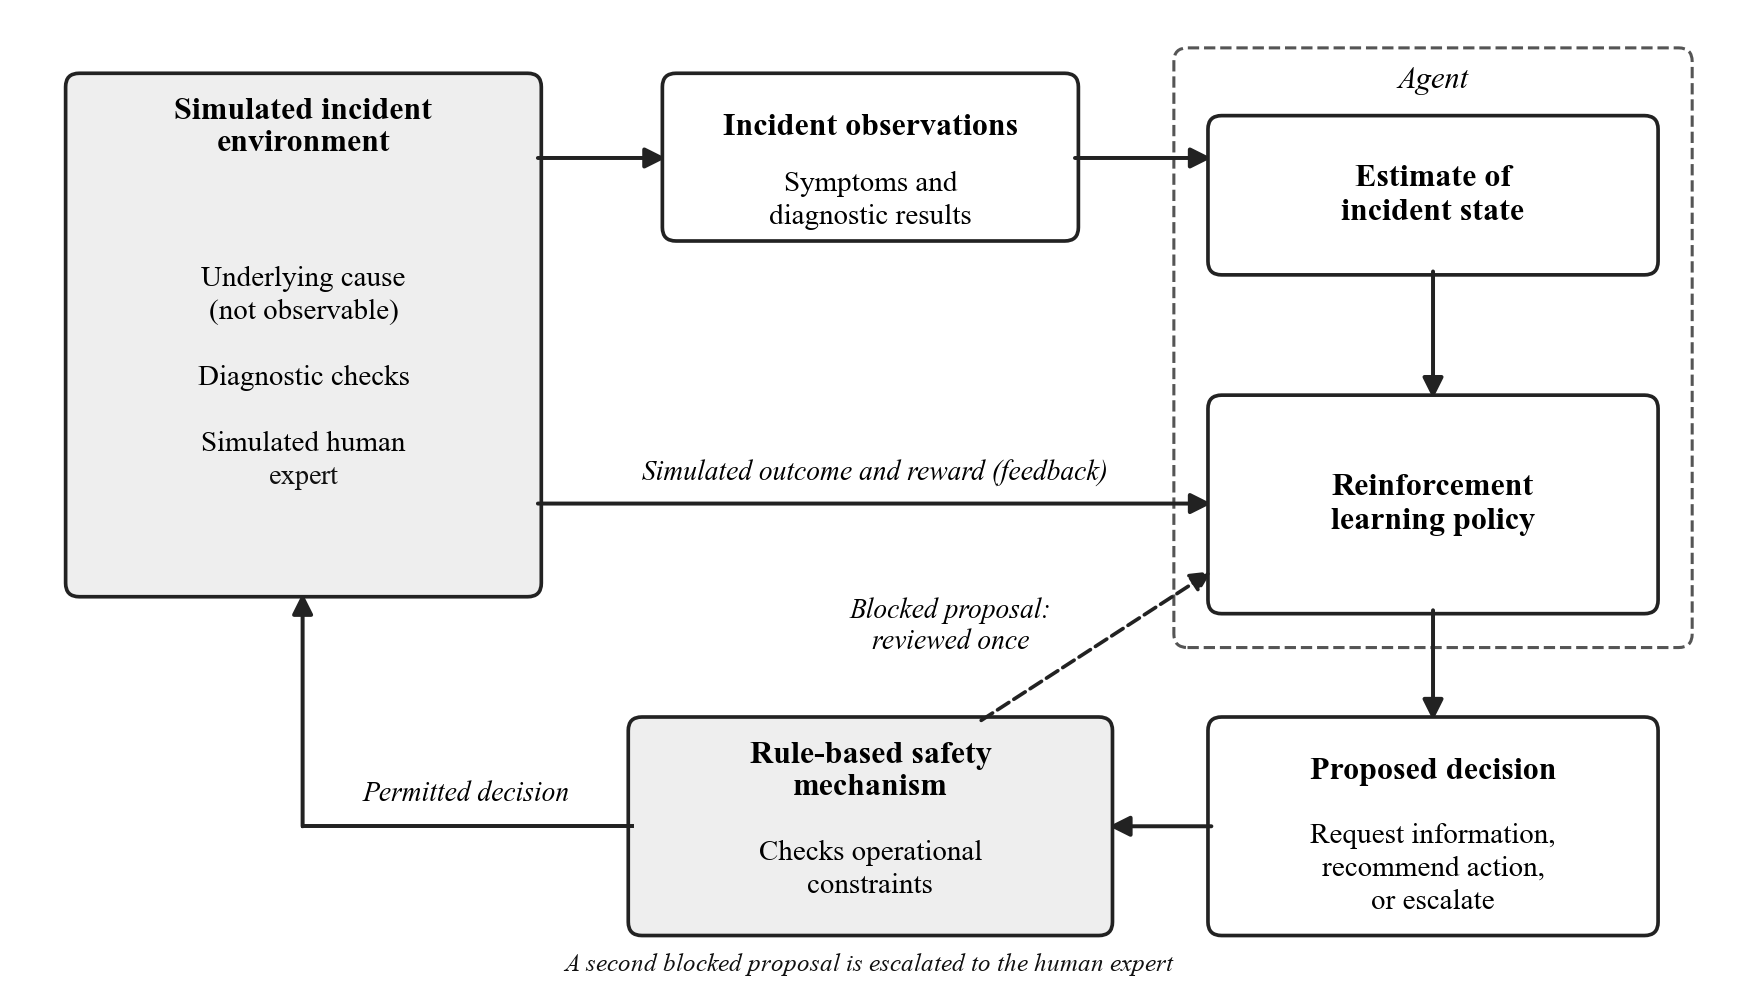
\includegraphics[width=\textwidth]{Figure_1_1_Conceptual_Framework.png}
\caption{Conceptual framework of the rule-constrained reinforcement learning agent for ambiguity-aware IT incident triage.}
\label{fig:framework}
\end{figure}

Each simulated incident has an underlying cause that the agent cannot observe directly. The agent receives incident observations instead: the initial symptoms and the results of any diagnostic checks it has requested. From these it maintains an estimate of the incident state, which summarises the evidence gathered so far. The reinforcement learning policy uses this estimate to propose one of three kinds of decision: request further diagnostic information, recommend an action, or escalate the incident to a human expert.

The independent rule-based safety mechanism checks every proposed decision against the predefined operational constraints before it takes effect. A proposal that satisfies the constraints passes to the environment unchanged, and a proposal that violates a constraint is blocked. The agent is told that its proposal was blocked and proposes again. If the second proposal also violates a constraint, the incident is escalated to the human expert. The environment then returns the simulated outcome. A diagnostic request returns new evidence at a cost, while a recommendation or an escalation ends the episode with an outcome that depends on the underlying cause. The reward derived from this outcome is the feedback from which the policy learns.

The framework separates learning from rule enforcement. The policy learns from feedback which permitted decision suits the evidence, and the safety mechanism enforces the rules regardless of what the policy has learned. The mechanism enforces only the constraints that have been specified, within the simulated environment, and the framework does not imply a guarantee of safety in real operations.

\section{Operational Definition of Key Terms}

\textbf{IT incident triage:} The early stage of incident handling in which a reported incident is assessed and a decision is made about what should happen to it next. In this study, triage is the decision among gathering more diagnostic information, recommending a permitted action, and escalating to a human expert.

\textbf{Ambiguity:} A condition in which the available evidence about an incident is consistent with more than one plausible cause, because the evidence is incomplete, uncertain, or conflicting.

\textbf{Incomplete diagnostic evidence:} Evidence from which one or more observations relevant to identifying the cause of an incident are missing at the time a decision is required.

\textbf{Reinforcement learning:} A machine learning approach in which an agent learns a decision policy by interacting with an environment and receiving rewards for the outcomes of its actions~\cite{sutton2018}. In this study, the environment is a simulation of IT incident triage.

\textbf{Diagnostic information gathering:} An action by which the agent requests an additional observation about an incident, such as the result of a diagnostic check, before committing to a recommendation or an escalation. Each request carries a cost in the simulation.

\textbf{Operational constraint:} A predefined rule that specifies an action the agent is not permitted to recommend, either in general or under stated conditions.

\textbf{Safety mechanism:} A rule-based component, independent of the learned policy, that checks each proposed action against the operational constraints and blocks actions that violate them. A blocked proposal is returned to the agent once, and a second blocked proposal results in escalation. It corresponds to the notion of a shield in safe reinforcement learning~\cite{alshiekh2018}. In this study, ``safety'' refers to compliance with the specified constraints and not to safety in a broader sense.

\textbf{Human escalation:} The decision to pass an incident to a human expert instead of recommending an action. In this study, the human expert is simulated.

\textbf{Baseline decision policy:} A simpler decision procedure against which the proposed agent is compared, such as a fixed rule-based policy or a reinforcement learning agent without the safety mechanism.

\section{Chapter Summary}

This chapter has introduced the study. It showed that IT incident triage often proceeds on incomplete or conflicting evidence, that existing automated approaches mostly treat triage as a single prediction, and that research on reinforcement learning, operational constraints and human deferral has developed largely apart. It stated the problem as the lack of evidence on how a rule-constrained reinforcement learning agent chooses among investigating, recommending and escalating under ambiguity, and it set out the objectives, research questions, hypotheses, scope, significance, justification, conceptual framework and key terms of the study, and it identified the Directorate of University ICT Services at Uganda Christian University as the setting for part of the work. Chapter Two reviews the related literature in greater depth and establishes the research gap more fully.


\chapter{Literature Review}
\label{ch:chapter-02}
% Chapter Two: Literature Review
% Compiled through main.tex; do not compile this file on its own.

\chapterheading{TWO}{LITERATURE REVIEW}

This chapter reviews the literature that bears on the five research questions of the study. It first describes how the literature was gathered and organised. It then synthesises the literature under five themes, one for each research question, and in each theme it separates what the reviewed studies establish from what they leave open. The chapter closes by comparing the studies closest to this one and by stating the research gap that the study addresses.

\section{Review Approach}

The review draws on three bodies of literature that Chapter One identified as relevant: AI-assisted IT incident management, safe and constrained reinforcement learning, and the deferral of decisions from automated systems to humans. A core set of 34 publications was collected across these areas. It comprises surveys of AIOps, empirical studies of incident management, foundational and recent work on shielding and constrained reinforcement learning, studies of selective prediction and learning to defer, and recent work on the runtime governance of language-model agents. Four further sources supply the standard formulations of reinforcement learning, partial observability, costly information acquisition and sequential deferral on which the discussion relies~\cite{sutton2018,kaelbling1998,janisch2019,joshi2023}.

A database search supplemented this core set. A search string combining three groups of terms, for the learning approach, for uncertainty and oversight, and for the incident-management setting, was run on Scopus, IEEE Xplore, the ACM Digital Library, SpringerLink and SIAM. The search returned 10,694 records with 10,541 distinct titles. These records were filtered by keyword for terms that denote IT operations and incident management. Seventy-seven records contained such terms in the title or abstract, and 19 of them referred specifically to incident management, incident response or AIOps. The abstracts of these records were read, and eight studies that addressed sequential decisions, information gathering, constraints or human involvement in incident handling were added to the review~\cite{alauthman2026,hammar2025,hammar2026llm,hammar2026belief,kim2025,dantonio2025,wang2023hrlhf,ding2023}. These eight studies are discussed on the basis of their abstracts, and the chapter attributes to them only what their abstracts state.

The synthesis is thematic. Each study was read for what it contributes to one or more of the research questions, and the findings were grouped into five themes that correspond to those questions: the representation of ambiguous incidents, sequential decisions about investigating, recommending and escalating, rule-based safety mechanisms, evaluation measures and baselines, and robustness under ambiguity. The review is therefore a structured thematic review of the collected literature. It does not claim the exhaustive coverage of a completed systematic review, and its conclusions about gaps are stated with that limit in mind.

\section{Representing Ambiguous Incident Triage in a Controlled Environment}

The first research question asks how ambiguous triage scenarios can be represented in a controlled environment. The literature answers part of this question by describing the evidence on which triage decisions rest. Remil et al.\ catalogue the data sources of incident management as incident reports, alerting signals, logs, metrics, traces and topology~\cite{remil2024}, and Zhang et al.\ add that language models have brought human-written material such as incident reports and documentation into use~\cite{zhang2025}. Incident reports are the primary source for the assignment of incidents~\cite{remil2024}. An environment for triage must therefore represent two kinds of evidence: the initial report, and the further observations that a member of IT staff could obtain from logs, metrics and other diagnostic sources.

The literature also explains why this evidence is ambiguous. Chen et al.\ found that distinct problems can produce similar symptoms, so that the symptoms alone do not identify the responsible team, and that incomplete knowledge of dependencies and imprecise assessment of resource health delay diagnosis~\cite{chen2020}. Remil et al.\ describe real IT data as commonly noisy and incomplete~\cite{remil2024}. Wu and Gong describe a related condition for agents that act in organisations: the facts needed to judge whether an action complies with policy may be absent from what the agent can see~\cite{wu2026}. Ambiguity in these accounts has three sources, which are missing observations, unreliable observations, and observations that are consistent with more than one cause. A controlled environment that claims to represent ambiguity should be able to produce each of them.

Realistic incident data is difficult to obtain, and this limits how the reviewed studies represent the task. Chen et al.\ report their results as relative values because of company policy~\cite{chen2020}. Remil et al.\ observe that publishing datasets raises confidentiality concerns, and that most methods for assignment and deduplication have been developed on software bug reports and not on operational incidents~\cite{remil2024}. Studies of sequential decision-making have responded by building or borrowing controlled environments. Dunsin et al.\ built a laboratory of infected virtual machines~\cite{dunsin2025}, Hammar and Li evaluated on the CAGE-2 benchmark~\cite{hammar2025}, Kim and D\'{a}n used simulations on synthetic and real dependency graphs~\cite{kim2025}, and Wang et al.\ combined production data with synthetic datasets containing injected anomalies~\cite{wang2023hrlhf}. Ren et al., in contrast, trained on a fixed dataset of recorded security incidents~\cite{ren2025}. Simulation is thus an accepted response to the scarcity of data, but the available environments model cyberattacks and microservice faults and not the triage of IT service incidents.

The formal tools for representing uncertainty about an incident are well established. A Markov decision process describes a decision problem in which the agent observes the state~\cite{sutton2018}, and a partially observable Markov decision process extends it to the case in which the agent receives only observations and must maintain a belief about the state~\cite{kaelbling1998}. Several incident-response studies adopt this view. Hammar et al.\ estimate a belief with particle filtering~\cite{hammar2026belief}, Kim and D\'{a}n maintain a belief in a hidden Markov model~\cite{kim2025}, and Alauthman et al.\ augment the state with recent telemetry and alert history to mitigate partial observability~\cite{alauthman2026}. These studies show that a hidden cause with noisy observations is a workable representation of an incident.

Taken together, the literature supplies the ingredients for representing ambiguous triage but not the representation itself. It identifies the evidence sources, explains the origins of ambiguity, and offers a formal model for hidden causes. What the reviewed studies do not provide is an environment for IT service incidents in which the level of ambiguity can be set deliberately and in which the available actions are those of triage. The first objective of this study responds to that absence.

\section{Reinforcement Learning for Investigating, Recommending and Escalating}

The second research question concerns how reinforcement learning can support the choice among gathering information, recommending an action and escalating. Research on incident triage has so far framed the task mainly as supervised prediction. The methods surveyed by Remil et al.\ range from Naive Bayes classifiers over report text to convolutional and recurrent networks that recommend a responsible team~\cite{remil2024}, and the triage component described by Chen et al.\ is a recurrent model over the incident text and discussion~\cite{chen2020}. One line of this work treats triage as a continuing process and updates its prediction as engineers add to the discussion~\cite{remil2024,chen2020}. The model in that case benefits from new evidence but does not decide to seek it. Zhang et al.\ add that automation in this field mainly stops at triage or the recommendation of solutions~\cite{zhang2025}. Where agents have been placed in the incident workflow, as in the runbook assistant that D'Antonio and Xie studied over 232 production incidents, the agent guides a human operator who carries out the mitigation~\cite{dantonio2025}. The triage literature therefore predicts well-defined labels but does not model the decision about what to do when the label is uncertain.

Reinforcement learning has entered IT operations and incident handling, mostly for diagnosis and response. Ding et al.\ learn a policy that prunes a service dependency graph before root cause analysis~\cite{ding2023}, and Wang et al.\ use hierarchical reinforcement learning to reduce the number of questions put to engineers when that graph is constructed~\cite{wang2023hrlhf}. In cybersecurity, Ren et al.\ train an agent to select response strategies~\cite{ren2025}, Dunsin et al.\ train an agent to conduct a malware investigation~\cite{dunsin2025}, and Alauthman et al.\ propose a deep Q-network agent for incident response in industrial control systems~\cite{alauthman2026}. Hammar and colleagues treat incident response as planning under partial observability~\cite{hammar2025,hammar2026belief}. These studies establish that sequential formulations of incident handling are feasible and can outperform fixed procedures in their own settings. Their action sets, however, consist of responses or investigative steps, and the studies do not address triage as defined in this study.

The decision to gather information has been studied as a sequential problem in its own right. Under partial observability, an action may be chosen for the information it yields, and its value depends on what that information costs~\cite{kaelbling1998}. Janisch et al.\ trained an agent to acquire costly features one at a time before classifying~\cite{janisch2019}. In incident handling, Kim and D\'{a}n choose which alerts to investigate so as to reduce the uncertainty of a belief~\cite{kim2025}, the agent of Dunsin et al.\ collects forensic evidence step by step~\cite{dunsin2025}, and Wang et al.\ learn which questions to ask engineers~\cite{wang2023hrlhf}. Information gathering is consequently a tractable learning problem, and one that has already been applied to parts of incident handling. In these studies the alternative to gathering information is to conclude, and none of them offers the agent the further option of passing the case to a person.

The decision to hand a case to a human has been studied separately, and mostly as a single-step choice. Selective prediction allows a model to abstain when its confidence is low~\cite{geifman2019}, and learning to defer trains a model to pass a case to a human decision-maker by taking that person's ability into account~\cite{madras2018,hemmer2023}. Strong et al.\ note that the standard formulation treats cases as independent and optimises a one-step outcome~\cite{strong2025}. Sequential extensions exist. Joshi et al.\ place deferral in a Markov decision process, where deferring affects later states~\cite{joshi2023}, and Zhang et al.\ formulate deferral as a constrained Markov decision process that accounts for the fatigue of the human expert~\cite{zhang2026falcon}. Guidance on AI risk management likewise lists deferral to a human expert among the configurations in which an AI system may operate~\cite{nist2023}. Applied work treats escalation as an estimate of when a model is likely to be wrong~\cite{bachar2026} or as a decision that policy can make mandatory~\cite{pacella2026}. In each case the choice is between acting and deferring, and the option of first gathering more evidence is absent.

The two lines of work thus stop on either side of the choice this study examines. Information-gathering studies offer the agent two options, to look further or to decide, and deferral studies offer two different options, to decide or to hand over. Hammar et al.\ come closest to joining them: their language-model planner abstains when its candidate actions are inconsistent and then collects external feedback, for example from a digital twin~\cite{hammar2026llm}. That system gathers feedback from a model of the system and not from a human, and its decision rule is a consistency threshold and not a learned policy. Among the reviewed studies, none trains a single policy to choose among investigating, recommending and escalating in IT incident triage.

\section{Rule-Based Safety Mechanisms and Operational Constraints}

The third research question asks how effectively a rule-based mechanism can prevent actions that violate operational constraints. Safe reinforcement learning offers two broad ways to impose constraints on a learning agent. Garc\'{\i}a and Fern\'{a}ndez divide the field into methods that modify the optimality criterion and methods that modify the exploration process with external knowledge~\cite{garcia2015}. Constrained policy optimisation belongs to the first group and bounds the expected cumulative cost of a policy~\cite{achiam2017,wachi2024}. Zhao et al.\ point out that many practical constraints are instead instantaneous and deterministic and must hold in every state~\cite{zhao2023}. An operational rule that forbids a particular action under stated conditions is a constraint of this second kind, which an expected-cost bound does not enforce.

Shielding enforces constraints of that kind by separating the rule from the learner. Wen et al.\ first computed a permissive strategy that satisfies a temporal logic specification and then let the agent learn within it~\cite{wen2015}. Alshiekh et al.\ generalised the idea into a shield that is synthesised from a specification and an abstraction of the environment, and that either restricts the actions offered to the agent or replaces an unsafe action after the agent selects it~\cite{alshiekh2018}. Later work relaxed the requirement of absolute safety. Jansen et al.\ block an action only when it raises the probability of a violation beyond a threshold~\cite{jansen2020}, and Yang et al.\ use probabilistic logic to handle noisy observations~\cite{yang2023}. Hamel-De le Court and colleagues have addressed scalability and uncertainty in the environment model~\cite{hamel2025,hamel2026}. K\"{o}nighofer et al.\ summarise the benefits of shielding as assured compliance with the specification, permissiveness towards safe actions, and preserved convergence of the learner~\cite{konighofer2025}.

Shielding has costs that matter for this study. A shield requires a formal model of the safety-relevant part of the environment, and its guarantee extends only as far as that model and the specification are correct~\cite{konighofer2025}. Pranger and K\"{o}nighofer observe that shielding has seen limited use in practice because it demands expertise in formal methods and considerable engineering effort~\cite{pranger2026}. Yang et al.\ note that a shield which simply rejects actions can hinder learning, because the agent is unaware that its choices were overridden~\cite{yang2023}. The demonstrations in this literature are grid worlds, arcade games, simulated robots and control tasks~\cite{alshiekh2018,jansen2020,achiam2017}. The method is therefore well understood in principle, while its use on the rule sets of IT operations remains largely unexamined.

A parallel body of work enforces explicit rules on language-model agents at run time. Wang et al.\ define a rule language with triggers, predicates and enforcement actions~\cite{wang2025agentspec}, Xiang et al.\ and Chen et al.\ use a second agent to check the actions of the first against stated policies~\cite{xiang2025,chen2025shieldagent}, and Pacella et al.\ place a policy-derived guardrail beneath the agent so that it cannot fall below the escalation that policy requires~\cite{pacella2026}. Wu and Gong check each proposed action against organisational state and return one of three verdicts, to allow, to block or to ask for clarification~\cite{wu2026}. Hu et al.\ show the scale that rule sets can reach, with a dataset of 12,985 rules drawn from 74 regulations and policies~\cite{hu2026}. This work confirms that rules kept outside the decision-maker can be inspected and enforced independently. It concerns language-model agents and not reinforcement learning, and it does not study how enforcement interacts with a policy that is still learning.

Two studies bring rule enforcement into incident response itself. Alauthman et al.\ couple their deep Q-network agent with an explicit safety shield that enforces operational constraints, in a design where the agent remains advisory by default and the operator can override it~\cite{alauthman2026}. Hammar et al.\ check the candidate actions of a language model for consistency with system constraints~\cite{hammar2026llm}. The first of these is the closest precedent for the mechanism proposed in this study, and it shows that the combination of a learned policy and a rule-based shield has been proposed for incident response. Its setting is cyber-physical control systems, its agent selects responses and does not choose whether to investigate or escalate, and its abstract reports an evaluation plan with indicative findings.

The literature therefore supports the feasibility of an independent rule-based mechanism and identifies the questions that remain. It is established that explicit rules can be enforced on a learning agent without preventing it from learning. It is less clear what should replace a blocked proposal when the agent's alternatives include requesting information and escalating, and how often a learned triage policy would propose prohibited actions in the first place. The third objective of this study addresses these questions for IT incident triage.

\section{Evaluation Measures and Baseline Policies}

The fourth research question concerns how the proposed approach should be compared with baseline policies. Each strand of the literature has its own measures. AIOps research evaluates triage with classification and ranking metrics and evaluates the process with time-based measures such as mean time to repair and mean time to engage~\cite{remil2024}. Remil et al.\ criticise the reliance on contingency-table metrics that ignore context and time~\cite{remil2024}, and Zhang et al.\ report that generated diagnoses and mitigation suggestions often require human assessment because they lack a fixed ground truth~\cite{zhang2025}. Reinforcement learning studies of incident response report the effectiveness of the response, the time taken, and false positive rates~\cite{ren2025}, or the time and accuracy of an investigation~\cite{dunsin2025}. These measures describe whether the final decision was correct and how quickly it was reached.

Studies of constraints and of deferral measure different things. Shielding studies compare a shielded agent with the same agent unshielded and report safety violations alongside reward~\cite{alshiekh2018,jansen2020}. Research on language-model agents has introduced measures that combine the two: Levy et al.\ credit a task only when it is completed without violating any applicable policy, and they find that this measure falls well below the raw completion rate for the agents they test~\cite{levy2026}. Mohammadi et al.\ list compliance with policy among the objectives that agent evaluation in enterprises must cover~\cite{mohammadi2025}. Deferral studies report accuracy as a function of coverage~\cite{geifman2019}, the accuracy of the combined human and model~\cite{madras2018}, or the trade-off between accuracy and the cost of human review~\cite{bachar2026}. Pacella et al.\ measure the recall of mandatory escalations and the stability of the decision across runs~\cite{pacella2026}. Turan relates the escalation rate to realised safety and argues that the relationship need not be monotonic~\cite{turan2026}.

The baselines used in these studies follow a common pattern. Learned policies are compared with fixed rule-based procedures~\cite{ren2025,pacella2026}, constrained agents with their unconstrained counterparts~\cite{alshiekh2018,jansen2020,pacella2026}, and deferring systems with the model alone and the human alone~\cite{madras2018,zhang2026falcon}. Dunsin et al.\ compare their agent with human experts~\cite{dunsin2025}. These comparisons isolate one property at a time, which is the contribution of learning, of the constraint, or of deferral.

No reviewed study reports all four kinds of measure for one agent. Decision quality, the cost of investigation, escalation behaviour and constraint compliance are each measured somewhere in the literature, but in different studies and for different systems. An agent that can investigate, recommend and escalate could score well on any one of them by neglecting the others, for example by escalating every case or by investigating without limit. The literature thus provides the individual measures and the baseline patterns that this study needs, and it leaves open how they behave when reported together. The fourth objective takes up that question.

\section{Robustness under Ambiguity and Missing Evidence}

The fifth research question asks how robust the approach is as evidence becomes incomplete, conflicting or more ambiguous. The literature treats robustness to imperfect data as a requirement. Remil et al.\ list it among the properties that AIOps solutions must have~\cite{remil2024}, and Mohammadi et al.\ treat robustness to variation as part of the reliability that agent evaluation should probe~\cite{mohammadi2025}. Some studies test it directly. Kim and D\'{a}n report that their investigation policies remain effective under high false-alert rates and investigation errors~\cite{kim2025}, and Hammar and Li evaluate response planning when the assumed model of the incident is wrong~\cite{hammar2025}. Ren et al.\ acknowledge that their agent generalises less well to attack patterns unlike those in its training data~\cite{ren2025}. These results concern the quality of the final decision as conditions degrade.

Uncertainty also affects the mechanisms that are meant to keep an agent within bounds. A deterministic shield assumes that the agent's observations are accurate, an assumption Yang et al.\ describe as unrealistic~\cite{yang2023}, and a shield computed from an estimated model can lose its guarantee when the estimate is wrong~\cite{hamel2026}. Wu and Gong show that a rule cannot be applied correctly when the facts it depends on are hidden from the checker~\cite{wu2026}. A rule-based mechanism in triage faces the same difficulty, because a rule whose condition refers to the state of a system can only be evaluated on the evidence available.

The human side of escalation is not constant either. Learning when to defer depends on data about the expert that is costly to obtain~\cite{hemmer2023}, people decide differently when they know that a model has deferred to them~\cite{bondi2022}, and expert accuracy changes with workload~\cite{zhang2026falcon}. Turan argues from a modelling study that increasing the escalation rate can reduce realised safety once the reviewer is overloaded~\cite{turan2026}. An agent that responds to ambiguity only by escalating more would therefore transfer the problem and not resolve it.

The reviewed studies have not examined how the balance among investigating, recommending and escalating shifts as ambiguity rises. Robustness has been measured for the accuracy of a decision, for the validity of a shield, and for the reliability of a human reviewer, each in isolation. For a triage agent, the behaviour of interest is the change in its mix of decisions: whether it investigates more, escalates more, or continues to recommend with less support. The fifth objective of this study measures that change across controlled levels of ambiguity and missing evidence.

\section{Synthesis of the Reviewed Literature}

Across the five themes the literature shows a consistent pattern: the components that this study needs exist, but they have been developed and evaluated apart. AIOps research describes the triage task and its evidence but models it as prediction. Reinforcement learning research on incident handling models sequential decisions but concentrates on response and investigation in cybersecurity. Shielding research provides a way to enforce rules on a learning agent but has been demonstrated mainly on control tasks. Deferral research explains when a model should hand a decision to a person but treats the hand-over mostly as a single-step alternative to prediction.

Table~\ref{tab:comparison} compares the studies closest to this one against the capabilities that the research questions concern. The comparison shows that each capability appears in at least one study and that the studies cluster in pairs of capabilities. Sequential policies are combined with information gathering~\cite{dunsin2025,kim2025,wang2023hrlhf}, or with a rule check~\cite{alauthman2026}, or with deferral~\cite{zhang2026falcon}. Rule checks are combined with escalation where the decision-maker is a language model~\cite{pacella2026}. No row other than the proposed study combines a sequential policy, information gathering, a rule check and human escalation, and none of the studies of IT service incidents includes a rule check or an escalation decision.

\begin{table}[htbp]
\centering
\caption{Comparison of the studies closest to this research. \cellyes~=~addressed; \cellpart~=~partly addressed; \cellno~=~not addressed or not reported. Studies marked $\dagger$ were assessed from their abstracts.}
\label{tab:comparison}
\small
\setlength{\tabcolsep}{4pt}
\begin{tabularx}{\textwidth}{@{}l>{\raggedright\arraybackslash}Xccccc@{}}
\toprule
Study & Setting & \rotatebox{70}{Sequential policy} & \rotatebox{70}{Information gathering} & \rotatebox{70}{Rule check} & \rotatebox{70}{Human escalation} & \rotatebox{70}{Varied ambiguity} \\
\midrule
Chen et al.~\cite{chen2020} & IT incident triage & \cellno & \cellno & \cellno & \cellno & \cellno \\
Wang et al.~\cite{wang2023hrlhf}$^\dagger$ & Root cause analysis & \cellyes & \cellyes & \cellno & \cellpart & \cellno \\
Ren et al.~\cite{ren2025} & Security incident response & \cellyes & \cellno & \cellno & \cellno & \cellno \\
Dunsin et al.~\cite{dunsin2025} & Malware investigation & \cellyes & \cellyes & \cellno & \cellno & \cellno \\
Kim and D\'{a}n~\cite{kim2025}$^\dagger$ & Security alert prioritisation & \cellyes & \cellyes & \cellno & \cellno & \cellyes \\
Hammar and Li~\cite{hammar2025}$^\dagger$ & Security incident response & \cellyes & \cellno & \cellno & \cellno & \cellyes \\
Hammar et al.~\cite{hammar2026llm}$^\dagger$ & Security response planning & \cellpart & \cellpart & \cellyes & \cellno & \cellno \\
Alauthman et al.~\cite{alauthman2026}$^\dagger$ & Industrial control incident response & \cellyes & \cellno & \cellyes & \cellpart & \cellno \\
Zhang et al.~\cite{zhang2026falcon} & Classification with deferral & \cellyes & \cellno & \cellno & \cellyes & \cellno \\
Pacella et al.~\cite{pacella2026} & Employee onboarding workflow & \cellno & \cellno & \cellyes & \cellyes & \cellno \\
Wu and Gong~\cite{wu2026} & Workplace assistant actions & \cellno & \cellpart & \cellyes & \cellno & \cellno \\
\midrule
This study (proposed) & IT incident triage & \cellyes & \cellyes & \cellyes & \cellyes & \cellyes \\
\bottomrule
\end{tabularx}
\end{table}

The comparison also qualifies any claim to novelty. A reinforcement learning agent with a safety shield has been proposed for incident response in industrial control systems~\cite{alauthman2026}, and a planner that checks its actions against constraints and seeks further feedback when uncertain has been evaluated for security incidents~\cite{hammar2026llm}. This study does not introduce the idea of constraining a learned incident-handling agent. Its contribution lies in the particular decision it studies, the setting in which it studies it, and the way it evaluates the result.

\section{Research Gap}

The review identifies five related gaps, one under each research question. The first is a gap in representation. The reviewed studies explain why triage evidence is ambiguous and provide formal models for hidden causes, but they offer no controlled environment for IT service incidents in which ambiguity can be varied and in which the actions are those of triage. The available environments model cyberattacks and microservice faults~\cite{hammar2025,dunsin2025,wang2023hrlhf}.

The second gap concerns the decision itself. Information-gathering studies let an agent choose between looking further and deciding~\cite{janisch2019,kim2025}, and deferral studies let it choose between deciding and handing over~\cite{madras2018,joshi2023,zhang2026falcon}. No reviewed study trains one policy to choose among all three options for IT incident triage. It is consequently unknown whether an agent can learn to treat investigation and escalation as distinct responses to uncertainty, or whether it will collapse into one of them.

The third gap concerns the interaction between rules and that decision. Rule-based shields have been shown to restrict learned policies in control tasks~\cite{alshiekh2018,konighofer2025}, and one study proposes a shield for incident response~\cite{alauthman2026}. The reviewed literature does not report how an independent rule-based mechanism behaves when the constrained agent can also request information or escalate, nor how often a learned triage policy proposes actions that the rules prohibit.

The fourth and fifth gaps concern evidence. Decision quality, investigation cost, escalation behaviour and constraint compliance have each been measured, but not together for one agent, so the trade-offs among them have not been observed. Robustness has been tested for decision accuracy and for the validity of shields~\cite{kim2025,hammar2025,hamel2026}, but not for the mix of investigating, recommending and escalating as ambiguity increases.

This study addresses these gaps within stated limits. It will construct a simulated environment for ambiguity-aware IT incident triage, train a rule-constrained reinforcement learning agent to choose among gathering diagnostic information, recommending a permitted action and escalating to a human expert, and evaluate the agent against baseline decision policies on all four measures and across levels of ambiguity. The gaps are stated for the literature reviewed in this chapter. Related work may exist beyond it, and the claim made here is that the reviewed literature leaves these questions open, not that they have never been examined.

\section{Chapter Summary}

This chapter reviewed the literature under five themes that correspond to the research questions of the study. It showed that the literature explains the sources of ambiguity in triage and supplies formal models for it, that sequential decision methods have been applied to incident response and investigation but not to the three-way choice of triage, that rule-based mechanisms can constrain learning agents but have rarely been examined in IT operations, and that evaluation measures and robustness tests exist separately for each strand. A comparison of the closest studies showed that none combines a sequential policy, information gathering, a rule check and human escalation, and the chapter stated five gaps on that basis. Chapter Three presents the methodology by which the study addresses them.


\chapter{Methodology}
\label{ch:chapter-03}
% Chapter Three: Methodology
% Compiled through Opol_Charis_Thesis.tex; do not compile this file on its own.

\chapterheading{THREE}{METHODOLOGY}

This chapter describes how the study will be carried out. It presents the research design and the pipeline of the project, and then describes each component in turn: the modelling of incident scenarios, the simulated triage environment, the reinforcement learning agent, the rule-based safety mechanism and the baseline decision policies. It then defines the evaluation metrics and the experiments, and closes with the tools, the threats to validity and the ethical considerations of the study. The chapter describes planned work, and it reports no results.

\section{Research Design}

The study follows a design-and-evaluate approach. It constructs an artefact, a rule-constrained reinforcement learning agent together with the environment in which the agent operates, and it evaluates that artefact through controlled experiments. This corresponds to the design science view of research in information systems, in which knowledge is produced by building an artefact that addresses an identified problem and by evaluating it rigorously~\cite{hevner2004}. The design suits the research questions, which ask how a task can be represented, how a method can be applied to it, and how well the result performs.

The evaluation is experimental and quantitative, and it is conducted entirely in simulation. Chapter Two showed that realistic incident data is scarce and confidential and that simulation is the accepted response in studies of sequential decision-making for incident handling~\cite{remil2024,hammar2025,dunsin2025}. Simulation also gives the study control over the variable of interest. The level of ambiguity can be set, held constant and varied, which would not be possible with live incidents. The cost of this choice is that the findings describe the behaviour of the agent under the assumptions of the simulator, a limit that Section~\ref{sec:validity} discusses.

A qualitative component informs the simulation. The Directorate of University ICT Services at Uganda Christian University has agreed to support the study, and its practice is the source from which the incident scenarios and operational rules are drawn. An initial semi-structured interview with a senior developer of the Directorate, held on 19 October 2026, described the current handling of incidents: users or support staff raise tickets, which are vetted and assigned to the responsible developer or, where that person is not known, to a senior developer; application errors are observed through system logs and a monitoring dashboard. The interviewee identified the application programming interface logs as the most informative source of evidence. This consultation shaped the incident categories in Section~\ref{sec:scenarios} and the treatment of escalation as a hand-over to the responsible member of staff. Table~\ref{tab:alignment} shows how each specific objective is addressed by a component of the method and by a set of measures.

\begin{table}[htbp]
\centering
\caption{Alignment of the specific objectives with the method and the evaluation.}
\label{tab:alignment}
\small
\begin{tabularx}{\textwidth}{@{}p{0.27\textwidth}LL@{}}
\toprule
Objective & Method component & Evidence produced \\
\midrule
1. Identify and model ambiguous triage scenarios & Scenario elicitation and incident model (Sections~\ref{sec:scenarios} and~\ref{sec:environment}) & Scenario model reviewed by Directorate staff \\
2. Design the reinforcement learning environment & Simulated triage environment and agent (Sections~\ref{sec:environment} and~\ref{sec:agent}) & Working environment; learning curves \\
3. Implement the rule-based safety mechanism & Safety mechanism (Section~\ref{sec:mechanism}) & Constraint compliance measures \\
4. Evaluate against baseline policies & Baselines, metrics and Experiments 1 to 3 (Sections~\ref{sec:baselines} to~\ref{sec:experiments}) & Decision quality, investigation efficiency, escalation behaviour, constraint compliance \\
5. Assess robustness under ambiguity & Experiment 4 (Section~\ref{sec:experiments}) & All measures across ambiguity levels \\
\bottomrule
\end{tabularx}
\end{table}

\section{Research Pipeline}

The project proceeds through eight phases, shown in Figure~\ref{fig:pipeline}. The first phase, the review of the literature and the specification of the problem, is reported in Chapters One and Two. The second phase elicits incident scenarios and operational rules with the Directorate. The third phase builds the simulated environment and tests it, and the resulting scenarios are returned to Directorate staff for review before they are fixed. The fourth and fifth phases implement the safety mechanism and the baseline policies. The sixth phase trains the agents, the seventh runs the experiments, and the eighth analyses and reports the results.

\begin{figure}[htbp]
\centering
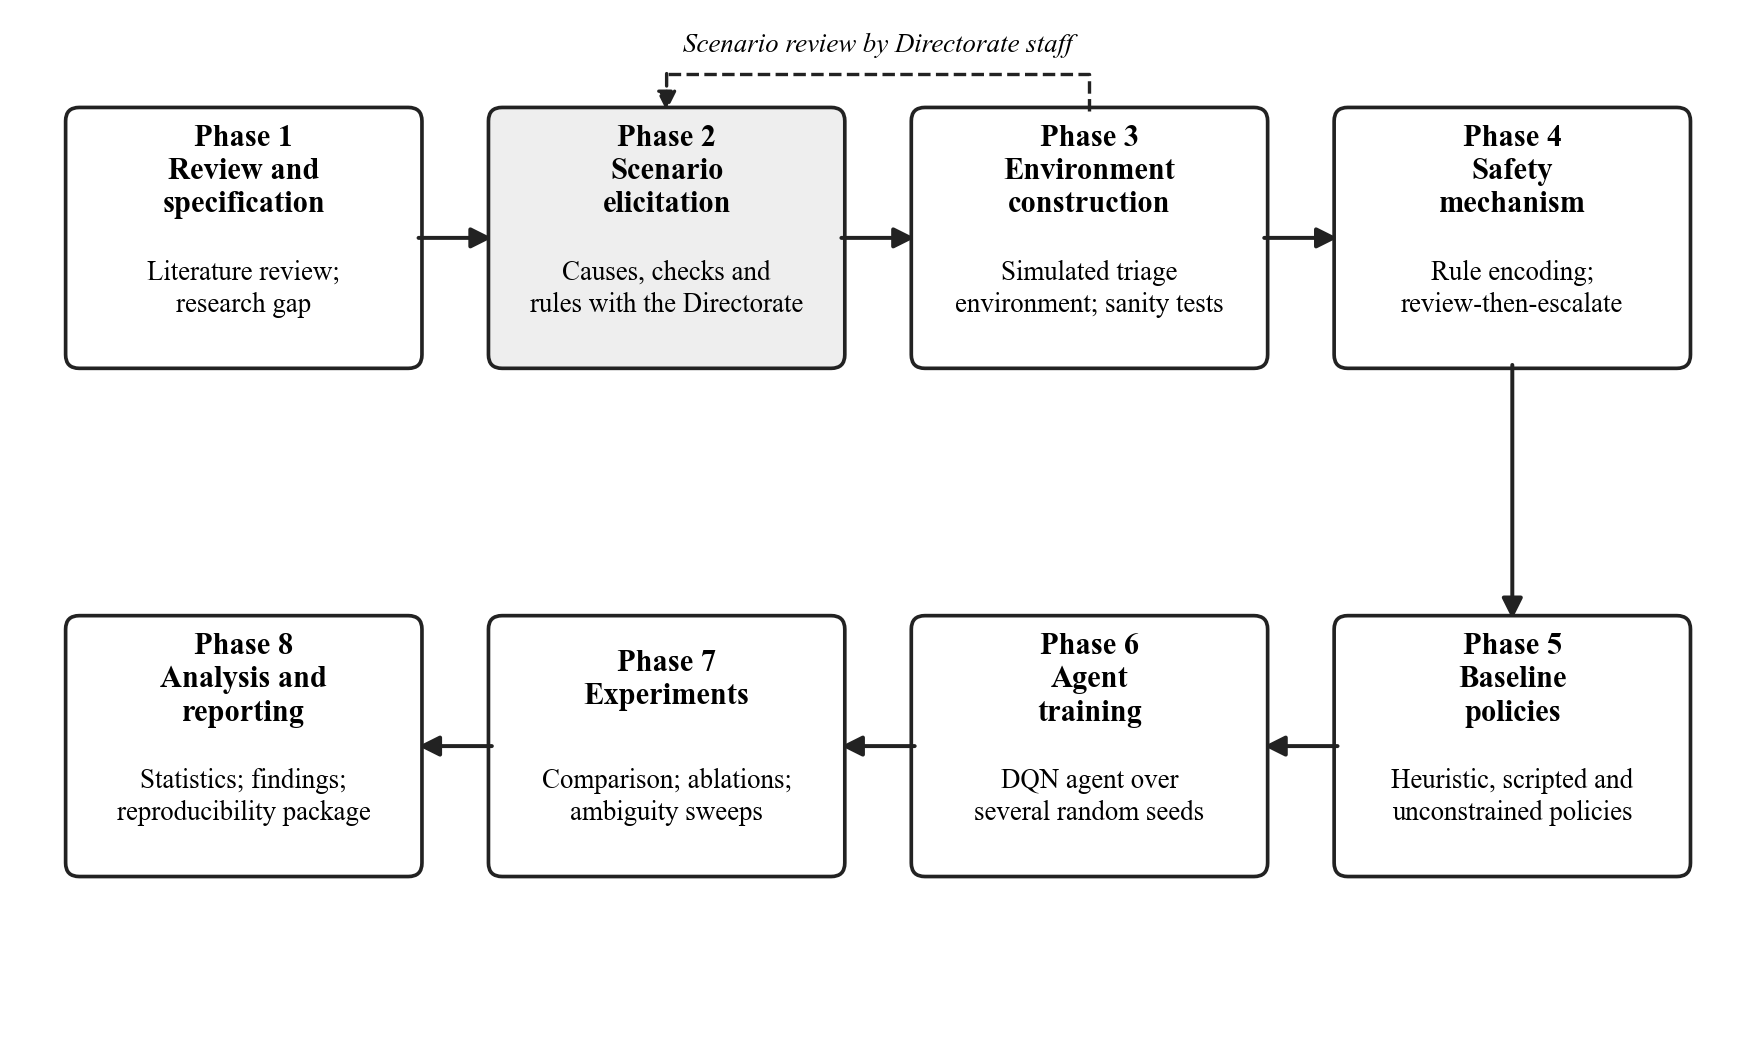
\includegraphics[width=\textwidth]{Figure_3_1_Research_Pipeline.png}
\caption{The research pipeline of the study.}
\label{fig:pipeline}
\end{figure}

The order of the phases reflects their dependencies. The environment cannot be built before the scenarios are specified, and the rules cannot be encoded before the actions and evidence they refer to exist in the environment. The baselines are implemented before the agent is trained so that the environment is exercised by simple policies first, which exposes errors in the simulator before they can be mistaken for properties of the learned agent.

\section{Scenario Modelling with the Directorate}
\label{sec:scenarios}

The scenario model defines what an incident is in the simulation. It consists of about 15 causes, 20 diagnostic checks and 10 operational rules. Fifteen causes is a target, not a limit: more are added if the Directorate can describe them well, since a smaller model that practitioners can rate and review with care is preferred to a larger one whose later entries are guesses. Following the initial consultation, the causes are drawn mainly from application errors observed in the logs of the university's systems, together with infrastructure causes that surface in those logs. They are distributed across four provisional categories: application and interface errors, authentication and access failures, database failures, and failures of infrastructure and external services. The categories are confirmed or revised in the elicitation. Each cause is associated with one remedy, which is the action that resolves an incident with that cause. Each check is a diagnostic observation that a member of IT staff could obtain, such as an entry in the application logs, a value on the monitoring dashboard, the result of reproducing a failing request or the state of a service, and each check has a cost that represents the effort of obtaining it. The symptoms correspond to what is first seen of an incident, such as the type of error and the affected function recorded in the logs, or the category of a user's ticket.

The content of the model is elicited from the Directorate. The elicitation seeks the causes of incidents that the Directorate encounters in these categories and the remedy for each, the symptoms with which those incidents are first reported, the checks that IT staff use to distinguish one cause from another, the rules that govern which actions may be taken and under what conditions, and the attributes of an incident to which those rules refer, such as whether the affected system is in production and the priority of the incident. The symptoms form a fixed list, so that each symptom is a named indicator and not free text. For each pair of cause and check, and for each pair of cause and symptom, the elicitation seeks a judgement of how likely the check or symptom is to be positive when that cause is present. It also seeks the approximate relative frequency of each cause and the effort required by each check. Where the Directorate can offer them, it seeks the relative costs of an escalation and of a wrong remedy and the frequency with which checks are unavailable or misleading; these inform the reward values and the ranges of the ambiguity controls but do not fix them. Any parameter that the elicitation does not supply is set by the researcher and reported as such.

The likelihoods are elicited on a five-point verbal scale, from \emph{never} through \emph{rarely}, \emph{sometimes} and \emph{often} to \emph{almost always}, which is mapped to the probabilities 0.05, 0.25, 0.5, 0.75 and 0.95. Asking for a verbal rating rather than a probability for each of the 300 pairs of cause and check keeps the task manageable for practitioners. Judgements are sought for the pairs that the Directorate considers related, and unrelated pairs take a default value that is reported with the model. The source of each judgement is recorded. These judgements become the parameters of the incident model described in Section~\ref{sec:environment}. The arrangements for the elicitation, including whether it draws on consultation with IT staff, on anonymised counts from the Directorate's ticketing and monitoring systems, or on both, are subject to the agreement reached with the Directorate. Such counts, for example of incidents by type and of the time taken to resolve them, would inform the relative frequency of each cause and the cost of an escalation.

The model is validated by expert review. After the environment has been built, sample incidents generated by the simulator are presented to Directorate staff, who judge whether the combinations of symptoms, check results and causes are plausible and whether the rules are stated correctly. The model is revised in response and then fixed before any agent is trained. Fixing the model before training prevents the scenarios from being adjusted, even unintentionally, in favour of the proposed agent.

The scenario model is a simplification, and the study states its simplifying assumptions. Each incident has exactly one cause, each cause has one correct remedy, and the result of a check does not change during an incident. Symptoms reach the agent as structured indicators from the elicited list; extracting them from the free text of a ticket is outside the scope of the study. These assumptions keep the model small enough to be specified and reviewed by people, at the cost of excluding incidents with several interacting causes and the errors that would arise in reading symptoms from text.

\section{The Simulated Triage Environment}
\label{sec:environment}

The environment casts triage as a sequential decision problem under partial observability. Chapter Two showed that a hidden cause with noisy observations is an established representation of an incident~\cite{kaelbling1998,kim2025,hammar2026belief}. The environment follows that representation and is implemented with the standard interface for reinforcement learning environments~\cite{towers2024}. One episode of the environment corresponds to the triage of one incident.

\subsection{Incident Model}

At the start of an episode the environment draws a cause $c$ from the set of causes $C = \{c_1, \dots, c_{K}\}$, where $K$ is the number of elicited causes (about 15), according to a prior distribution $P(c)$. The cause is hidden from the agent for the whole episode. The environment also draws a context for the incident, consisting of attributes such as whether the affected system is a production system and the priority of the incident. The context is visible to the agent, and the operational rules refer to it.

Evidence about the cause is generated by a likelihood model. Each diagnostic check $d_i$ in the set $D = \{d_1, \dots, d_{20}\}$ has a binary result, and the probability of a positive result depends on the cause:
\begin{equation}
\theta_{ij} = P(d_i = \text{positive} \mid c_j).
\label{eq:likelihood}
\end{equation}
The initial symptoms of the incident are generated in the same way from a set of symptom indicators, and they are revealed to the agent at the first step. The true result of every check is drawn once at the start of the episode, independently of the other checks given the cause, so that requesting a check twice returns the same result.

\subsection{Observations and State}

The agent never observes the cause. It observes an evidence vector that records, for each check, one of four values: not yet requested, unavailable, negative or positive. Each symptom indicator takes one of three values, present, absent or not reported, since all symptoms are revealed at the first step. The vector also contains the context attributes, the number of steps taken, and an indicator that is set when the previous proposal was blocked by the safety mechanism. This evidence vector is the agent's estimate of the incident state. Giving the learner access to the state of the safety mechanism follows Alshiekh et al., whose learner can base its actions on the state of the shield~\cite{alshiekh2018}.

The evidence vector is presented to the agent as a fixed-length vector of numbers. Each categorical value, namely the result of a check, the value of a symptom and each context attribute with more than two levels, is one-hot encoded, so that no artificial ordering is imposed on its values. Binary attributes and the blocked indicator take the values 0 and 1, and the number of steps is divided by the step limit so that it lies between 0 and 1. The length of the vector is fixed by the number of symptoms and context attributes established in the elicitation.

Because the results of checks do not change within an episode, the vector summarises everything the agent has learned about the incident, and the agent does not need a memory of earlier steps. Studies of incident response in which evidence arrives as a stream of events encode a history, with a transformer over recent security events~\cite{ren2025} or with recent telemetry and alert history~\cite{alauthman2026}, and a model of a fatiguing human expert uses a sequence model to track workload over an episode~\cite{zhang2026falcon}. The static evidence assumed here allows a feed-forward network to be used instead.

This choice does not give up the belief that a partially observable formulation requires. In the systematic review, the methods that kept an explicit belief over the hidden state were the most robust to model error and system change~\cite{opol2026slr,hammar2025,hammar2026belief}. In this environment the results of checks are fixed within an episode and independent of one another given the cause, and missing and reversed results arise independently of the cause. The posterior probability of each cause is then determined by the prior, the initial symptoms and the results observed so far, so the evidence vector is a sufficient statistic for the belief that a partially observable agent would maintain~\cite{kaelbling1998}. The agent does not compute that belief explicitly, because it is not given the likelihood model; it must learn the mapping from evidence to action. The threshold policy of Section~\ref{sec:baselines}, which is given the likelihood model and computes the posterior directly, serves as the explicit-belief reference.

\subsection{Actions}

The agent has $20 + K + 1$ actions, 36 with 15 causes. Twenty actions each request one diagnostic check, $K$ actions each recommend the remedy for one cause, and one action escalates the incident to a human expert. A request returns the result of the check and continues the episode. A check that has already been requested is removed from the agent's choices for the rest of the episode, since repeating it would return the same result. A recommendation or an escalation ends the episode. An episode also ends, as an escalation, if the agent reaches a fixed limit on the number of steps without deciding.

\subsection{Reward}

The reward expresses the costs that Chapter One attributed to each choice. A correct recommendation receives a positive reward $r_{\text{correct}}$. A wrong recommendation receives a penalty $-\lambda_{\text{wrong}}$. Each request for check $d_i$ incurs its cost $-k_i$. An escalation incurs a cost $-\lambda_{\text{esc}}$, which represents the expert's time. The values satisfy
\begin{equation}
r_{\text{correct}} > -\lambda_{\text{esc}} > -\lambda_{\text{wrong}},
\label{eq:reward}
\end{equation}
so that resolving an incident correctly is better than escalating it, and escalating it is better than recommending the wrong remedy. The simulated expert is assumed to resolve every escalated incident. The numerical values are set in pilot runs before the experiments begin and are reported with the results. Because the behaviour of the agent depends on these values, the study also examines how the results change when the cost of escalation is varied.

\subsection{Ambiguity Controls}
\label{sec:ambiguity}

Chapter Two identified three sources of ambiguity: missing observations, unreliable observations, and observations consistent with more than one cause. The environment has one control for each.

\begin{enumerate}
  \item \textbf{Missing evidence.} With probability $p_{\text{miss}}$, a check is unavailable for the whole episode, and a request for it returns the value ``unavailable''.
  \item \textbf{Unreliable evidence.} With probability $p_{\text{noise}}$, the result of a check is reversed before the agent receives it.
  \item \textbf{Overlapping evidence.} An overlap parameter $\omega$ between 0 and 1 moves the likelihood profile of each cause towards the average profile of its category, $\theta'_{ij} = (1 - \omega)\,\theta_{ij} + \omega\,\bar{\theta}_{i}$, where $\bar{\theta}_{i}$ is the mean of $\theta_{ij}$ over the causes in the same category as $c_j$. As $\omega$ increases, causes within a category become harder to tell apart.
\end{enumerate}

A setting of the three controls defines an ambiguity level. The base level, used for training and for the main comparison, is fixed in pilot runs so that the task is neither trivial nor impossible. The planned ranges for the robustness experiment are $p_{\text{miss}} \in \{0, 0.2, 0.4, 0.6\}$, $p_{\text{noise}} \in \{0, 0.1, 0.2, 0.3\}$ and $\omega \in \{0, 0.25, 0.5, 0.75\}$.

\subsection{Reference Labels}
\label{sec:labels}

The simulator knows the hidden cause and the likelihood model, so it can label each episode with the outcome that would have been appropriate. An incident is labelled as one that should be escalated in either of two cases. In the first, the operational rules prohibit the agent from recommending the remedy for the true cause in the context of the incident. In the second, the incident is irreducibly ambiguous: even with the result of every available check, the most probable cause under the simulator's own model is not the true cause. All other incidents are labelled as resolvable. These labels are used only for evaluation and are never shown to the agent.

The simulator is checked for leakage of the hidden cause before any agent is trained. Sahin and Mert found that an earlier version of their own simulator leaked the label into the agent's observations, so that any threshold appeared to achieve perfect recall~\cite{sahin2026}. In this environment no policy that sees only the observations can, on average, resolve correctly a larger share of incidents than the recommendation of the most probable cause after every available check, and by the definition above that share is the share of incidents labelled as resolvable. This ceiling is computed at each ambiguity level, and a learned or baseline policy whose resolution accuracy exceeds it by more than sampling error is taken as evidence of leakage, to be corrected before the experiments proceed.

\section{The Reinforcement Learning Agent}
\label{sec:agent}

The agent learns a policy that maps the evidence vector to one of the $20 + K + 1$ actions. The primary learning algorithm is the deep Q-network (DQN), which estimates the expected return of each action with a neural network~\cite{mnih2015}. Three considerations motivated the choice. First, the action set is small and discrete, which value-based methods handle directly. Second, the evidence vector admits $4^{20}$ combinations for the checks alone, which rules out the tabular Q-learning used in earlier incident-handling and shielding studies~\cite{dunsin2025,alshiekh2018} while retaining the same family of methods. Third, DQN yields an estimated value for every action, so the values the agent assigns to a blocked remedy and to escalation can be inspected when its behaviour is analysed. Constrained optimisers such as constrained policy optimisation and PPO-Lagrangian~\cite{achiam2017,zhang2026falcon} were not adopted, because they bound the expected cumulative cost of a policy, whereas the operational rules must hold at every step and are enforced by a separate mechanism (Section~\ref{sec:mechanism}). Policy-gradient methods are common in recent shielding studies~\cite{yang2023,konighofer2025}, and proximal policy optimisation~\cite{schulman2017} therefore serves as a secondary learner. Where time permits, the main comparison is repeated with it to show whether the findings depend on the choice of learner. Both algorithms are taken from an established open-source library to limit implementation error~\cite{raffin2021}. The library's DQN does not support action masking, so the removal of blocked actions and of checks already requested is implemented by restricting the choice of action, and the maximum in the learning target, to the available actions.

Each agent is trained by interaction with the environment at the base ambiguity level. Training begins from the library's default hyperparameters, and a small search over the learning rate, the network size and the exploration schedule is carried out on a set of random seeds that is not used in the final experiments. The training length is set from the pilot runs as the point at which the mean return stops improving. The final hyperparameters, the training length and the search itself are reported with the results.

A second training regime is used for the robustness question. In it the ambiguity controls are drawn at random from their planned ranges at the start of each episode, so that the agent meets many levels of ambiguity during training. Comparing the two regimes shows whether robustness requires exposure to ambiguity during training or carries over from training at a single level.

\section{The Rule-Based Safety Mechanism}
\label{sec:mechanism}

The safety mechanism is a component separate from the agent that checks every proposed action against the operational rules. Each rule is a condition over three things: the proposed action, the context of the incident, and the evidence gathered so far. A rule may, for example, prohibit a remedy on a production system, or prohibit a remedy until a named check has been observed. An action is prohibited if any rule prohibits it. Escalation is never prohibited, so a permitted action always exists. The ten rules are those elicited from the Directorate, encoded as explicit conditions that can be read and reviewed without reference to the agent.

The mechanism follows a review-then-escalate procedure when it blocks a proposal.

\begin{enumerate}
  \item The agent proposes an action. If no rule prohibits it, the action passes to the environment unchanged.
  \item If a rule prohibits the action, the mechanism blocks it and records the event. The step is consumed without reward. The agent receives the same evidence vector with the blocked indicator set, and the blocked action is removed from its choices for the next step.
  \item The agent proposes a second action. If it is permitted, it passes to the environment and the episode continues as normal.
  \item If the second proposal is also prohibited, the mechanism ends the episode by escalating the incident to the human expert. This outcome is recorded as a forced escalation.
\end{enumerate}

This design responds to three findings of Chapter Two. The first is that its central step has no precedent: of the 34 studies in the systematic review, only three report what replaces a blocked decision, by substitution, hand-off or deferral, and none gives the agent a second proposal~\cite{opol2026slr,ravi2025,singh2026,sahin2026}. The other two concern how the block is handled. A shield that silently replaces an action can hinder learning because the agent does not know that it was overridden~\cite{yang2023}; here the agent is told of the block and given one opportunity to choose again. Where a decision cannot be made within the rules, the appropriate fallback is to hand it to a person~\cite{pacella2026}; here a second block has that effect. The mechanism belongs to the family of shields that act after the agent has chosen~\cite{alshiekh2018}. It differs from them in that its rules are written directly and not synthesised from a formal model of the environment, so it carries no formal guarantee beyond the rules as written. Within the simulation it ensures that no prohibited action is executed.

\section{Baseline Decision Policies}
\label{sec:baselines}

No published system can be compared with the proposed agent directly, because the closest studies address other domains and share no environment with this one. The agent is therefore compared with baseline policies that run in the same environment, each standing for an approach identified in Chapter Two. Table~\ref{tab:baselines} lists them.

\begin{table}[htbp]
\centering
\caption{Baseline decision policies and the approaches they represent.}
\label{tab:baselines}
\small
\begin{tabularx}{\textwidth}{@{}p{0.2\textwidth}LL@{}}
\toprule
Policy & Behaviour & Approach represented \\
\midrule
Initial-symptom policy & Recommends the most probable cause given the initial symptoms, without requesting checks & Triage as a single prediction~\cite{chen2020,remil2024} \\
Scripted policy & Requests a fixed sequence of checks for the reported category and then recommends the most probable cause & Rule-based and runbook practice~\cite{remil2024,dantonio2025} \\
Always-escalate policy & Escalates every incident & The limiting case of deferral \\
Threshold policy & Maintains the posterior probability of each cause, requests the most informative check while no cause exceeds a confidence threshold, recommends when one does, and escalates when the checks are exhausted & Selective prediction and uncertainty-driven investigation~\cite{geifman2019,kim2025} \\
Unconstrained agent & The same learning agent trained and run without the safety mechanism & The standard comparison in shielding studies~\cite{alshiekh2018,jansen2020} \\
Penalty-only agent & The same learning agent without the mechanism, with a reward penalty for each prohibited action & Constraint by reward penalty~\cite{konighofer2025} \\
\bottomrule
\end{tabularx}
\end{table}

The order of checks in the scripted policy is elicited from the order in which Directorate staff examine evidence for each category of incident, so that the policy reflects current practice and not an arbitrary sequence. This matters because, in the systematic review, no extracted result showed a static baseline outperforming a learned policy, and weak baselines could not be ruled out as the reason~\cite{opol2026slr}. Where the elicitation does not supply an order for a category, the checks are ordered by their expected information about the cause under the elicited likelihoods, and this is reported.

Two of these baselines deserve comment. The threshold policy is given the simulator's likelihood model, which the learning agent must infer from experience. It is therefore a strong reference, and the study does not assume that the learned agent will exceed it. The always-escalate policy executes no prohibited action and makes no wrong recommendation, and it shows why no single measure can be read alone. The first four policies are run with the safety mechanism in place, so that their proposals are checked in the same way as those of the proposed agent.

Two ablations of the proposed agent complete the comparison. In the first, the agent cannot request checks and must recommend or escalate from the initial symptoms, which corresponds to the two-way choice studied in the deferral literature~\cite{madras2018}. In the second, the agent cannot escalate voluntarily and must gather evidence and then recommend, which corresponds to the two-way choice studied in the literature on information acquisition~\cite{janisch2019}. The ablations show what each option contributes to the three-way decision.

\section{Evaluation Metrics}
\label{sec:metrics}

Every policy is evaluated on the same fixed set of $N$ evaluation episodes at each ambiguity level. Each episode ends in a correct recommendation, a wrong recommendation or an escalation. Let $N_{\text{c}}$, $N_{\text{w}}$ and $N_{\text{e}}$ be the numbers of episodes with each outcome, so that $N = N_{\text{c}} + N_{\text{w}} + N_{\text{e}}$. The metrics are standard measures taken from the strands of literature reviewed in Chapter Two, and they are grouped under the four measures named in the fourth objective.

\subsection{Decision Quality}

Decision quality describes how often the agent's final decision is right. \emph{Resolution accuracy} is the share of all incidents that the agent resolves itself, $N_{\text{c}} / N$. It is the usual accuracy of the triage literature~\cite{remil2024}, and it penalises an agent that avoids error by escalating. \emph{Coverage} is the share of incidents on which the agent makes a recommendation, $(N_{\text{c}} + N_{\text{w}}) / N$, and \emph{selective accuracy} is the accuracy of those recommendations, $N_{\text{c}} / (N_{\text{c}} + N_{\text{w}})$. These two are the standard pair of selective prediction~\cite{geifman2019}. They are reported together because either can be raised at the expense of the other. The \emph{wrong-recommendation rate}, $N_{\text{w}} / N$, isolates the most costly error in triage. The \emph{mean episodic return} is the average total reward per episode. It is the quantity the agent is trained to maximise and the standard summary in reinforcement learning~\cite{sutton2018}, but it depends on the reward values chosen and is never reported alone.

\subsection{Investigation Efficiency}

Investigation efficiency describes what the agent spends on evidence before it decides. The \emph{mean number of checks} is the average number of requests per episode, and the \emph{mean investigation cost} is the average of the summed check costs per episode. The cost stands in for time, which a simulation without a clock cannot measure directly. The two are read together with accuracy as an \emph{accuracy--cost curve}, following the evaluation of costly feature acquisition~\cite{janisch2019}. The curve shows whether additional investigation yields additional accuracy and allows policies to be compared at equal cost.

\subsection{Escalation Behaviour}

Escalation behaviour describes how much the agent hands to the human expert and whether it hands over the right cases. The \emph{escalation rate} is $N_{\text{e}} / N$, the load placed on human experts~\cite{turan2026}. The remaining metrics use the reference labels of Section~\ref{sec:labels}. \emph{Escalation precision} is the share of escalated incidents that were labelled as ones that should be escalated; low precision means that human experts receive incidents the agent could have resolved. \emph{Escalation recall} is the share of incidents labelled as ones that should be escalated that the agent did escalate; low recall is the failure of under-escalation that Pacella et al.\ measured~\cite{pacella2026}. The \emph{escalation F1 score} is the harmonic mean of the two. Because precision, recall and F1 can all look acceptable when one class is rare, the \emph{escalation Matthews correlation coefficient} between the agent's choice to escalate and the reference label is also reported; it uses all four cells of the confusion matrix, and Okafor found that it exposed degenerate triage policies that F1 and ROC-AUC concealed~\cite{okafor2026}. Forced escalations are excluded from these three metrics and reported under constraint compliance, because they are produced by the mechanism and not chosen by the agent. Escalations caused by the step limit are likewise counted separately.

\subsection{Constraint Compliance}

Constraint compliance describes the agent's relationship to the rules. The \emph{proposed-violation rate} is the number of blocked proposals divided by the number of proposals. It shows whether the agent has learned to act within the rules or relies on being stopped. The \emph{forced-escalation rate} is the share of episodes that end with a second blocked proposal. The \emph{executed-violation rate} is the share of episodes in which a prohibited action takes effect. It is zero by construction when the mechanism is active, and it is the central measure for the unconstrained and penalty-only agents, as in the shielding literature~\cite{alshiekh2018,jansen2020}. The \emph{compliant success rate} is the share of episodes that end in a correct recommendation with no executed violation. It follows the measure of completion under policy introduced for agent benchmarks~\cite{levy2026}, and for agents without the mechanism it shows how much of their accuracy was obtained by breaking rules.

\subsection{Robustness}

Robustness is not a separate metric. Each metric above is computed at every ambiguity level and reported as a function of that level, in the manner of studies that vary false-alert rates or model error~\cite{kim2025,hammar2025}. Two views are reported. The first is degradation, the change in resolution accuracy and wrong-recommendation rate relative to the base level. The second is the decision mix, the coverage, the escalation rate and the mean number of checks at each level, which shows whether the agent responds to ambiguity by investigating more, by escalating more, or by continuing to recommend on weaker evidence.

\section{Experimental Design}
\label{sec:experiments}

The study comprises four experiments. Each learning agent is trained with ten random seeds, and results are reported as the mean over seeds with a 95\% bootstrap confidence interval, following recommended practice for reporting reinforcement learning results~\cite{agarwal2021}. The evaluation episodes are generated with seeds that are not used in training, and the same episodes are presented to every policy so that differences between policies are not due to differences between incidents. These choices answer the reporting weaknesses found in the systematic review, in which only 11 of 34 studies reported results over several runs with a measure of variance, nine tested their agents on conditions not seen in training, and five reported their hyperparameters and released their code or environment~\cite{opol2026slr}. This study reports variance over seeds, evaluates on unseen episodes and on ambiguity levels not used in training, and archives its code and configurations (Section~\ref{sec:tools}).

\textbf{Experiment 1: comparison with baselines.} The proposed agent is compared with the six baseline policies at the base ambiguity level on all metrics. This experiment addresses the fourth research question and the first hypothesis.

\textbf{Experiment 2: effect of the safety mechanism.} The proposed agent is compared with the unconstrained agent and the penalty-only agent on the constraint compliance metrics and on decision quality, and the proposed-violation rate is tracked over training. The two studies in the systematic review that measured a hard rule mechanism reached opposite results, one finding that the rules cost almost nothing~\cite{singh2026} and the other that they produced many false actions~\cite{ravi2025}, and neither reported how often blocked proposals occurred as training progressed. Tracking that rate shows whether the agent learns to act within the rules or continues to rely on being stopped. This experiment addresses the third research question and the second hypothesis.

\textbf{Experiment 3: ablation of the action set.} The proposed agent is compared with its two ablations to establish what the options to investigate and to escalate each contribute. This experiment addresses the second research question.

\textbf{Experiment 4: robustness.} All policies are evaluated across the planned ranges of the three ambiguity controls, varied one at a time from the base level and then jointly, for agents trained under both training regimes. This experiment addresses the fifth research question and the third hypothesis.

The first research question, on representation, is answered by the scenario model and the environment themselves and by their review by Directorate staff. A sensitivity analysis accompanies the experiments: the cost of escalation is varied around its chosen value and Experiment 1 is repeated, to show how far the conclusions depend on the reward design.

\section{Tools and Implementation}
\label{sec:tools}

The environment, the safety mechanism and the baselines are implemented in Python. The environment follows the Gymnasium interface~\cite{towers2024}, and the learning algorithms are those of Stable-Baselines3~\cite{raffin2021}. The scenario model, the rules and the settings of every experiment are held in configuration files and not in code, so that each result can be traced to the configuration that produced it. Random seeds are fixed and recorded. The code, the configurations and the evaluation episodes will be archived with the project so that the experiments can be repeated, with any material that the Directorate regards as confidential withheld or generalised.

\section{Validity and Limitations}
\label{sec:validity}

The main threat to the validity of the study is the realism of the simulator. The agent's behaviour is valid for incidents generated by the likelihood model, and that model rests on elicited judgements and on the simplifying assumptions of Section~\ref{sec:scenarios}. Expert review of generated incidents reduces this threat but does not remove it. The findings should therefore be read as evidence about the method under stated assumptions, and not as a prediction of performance on live incidents.

Three further limitations follow from design choices. First, the simulated expert resolves every escalated incident at a fixed cost. Chapter Two showed that the accuracy of human reviewers varies with workload~\cite{zhang2026falcon,turan2026}, so the study understates the cost of heavy escalation, and it reports the escalation rate so that this cost remains visible. Second, the results depend on the reward values, which the sensitivity analysis addresses only for the cost of escalation. Third, the safety mechanism enforces the rules as written, and it can only evaluate a rule on the evidence available; a rule that depends on a fact the agent has not observed cannot be applied correctly~\cite{wugong2026}.

The study also limits what it claims about generality. The scenario model reflects the practice of one organisation and four categories of incident, and the initial consultation drew on a single interview. Whether the findings hold for other organisations, other categories or larger models is a question for further work.

\section{Ethical Considerations}

The study will be conducted with the permission of the Directorate and in accordance with the research ethics requirements of the university. Participation by Directorate staff in the interviews, elicitation and review is voluntary, consent is obtained before any statement is used, and no member of staff is identified in the report. The initial consultation identified the security of incident data, including control over who can see it, as the main condition for using an agent of this kind; this is one reason the study works from elicited parameters in simulation and not from live data. Any incident records used to inform the scenario model are anonymised before use, and no personal data, credentials or confidential details of the university's systems appear in the simulator, the report or the archived materials. The agent is trained and evaluated only in simulation. It is not connected to any live system, and it executes no action on the infrastructure of the university.

\section{Chapter Summary}

This chapter described the methodology of the study. The study constructs a simulated triage environment from a scenario model of about 15 causes, 20 diagnostic checks and 10 operational rules elicited from the Directorate of University ICT Services, in which missing, unreliable and overlapping evidence can each be controlled. A reinforcement learning agent chooses among requesting checks, recommending remedies and escalating, and an independent rule-based mechanism reviews each proposal, returns a blocked proposal to the agent once, and escalates the incident if the second proposal is also blocked. The agent is compared with six baseline policies and two ablations on standard measures of decision quality, investigation efficiency, escalation behaviour and constraint compliance, across controlled levels of ambiguity. Chapter Four presents the implementation and the results of these experiments.


% ---------------------------------------------------------------------------
% References: one list for the whole document, numbered in order of citation.
% ---------------------------------------------------------------------------
\bibliographystyle{IEEEtran}
\bibliography{citations/references}
\addcontentsline{toc}{chapter}{REFERENCES}

\end{document}
